
\chapter{Methodology}

\label{Chapter5:Methodology} 
%----------------------------------------------------------------------------------------
%	SECTION 1
%----------------------------------------------------------------------------------------

In this Chapter we will discuss the entire work flow and the methods used in this study. Starting from the different model architecture and system setup describing various experimental configuration. We used two two main architecture and with some configurations to answer our research questions.


\section{System Overview}
We approached this problem of depth map estimation from monocular images to give end to end solution as much as possible using two CNN. As we discussed in the section \ref{Chapeter1:Topic_Description} our main focus was (a) to deliver a robust method and (b) regeneration of dead pixels or holes for better reconstruction of images. For this we consider two CNN models, first, we propose a model and this approach we call it as \textbf{A1} and the second model approach is a state of the art model and we call it as \textbf{A2}.  In this section we briefly describe both our models and input representation used for the experiments. And further more in order to improve our results we also propose different configuration methods. These configuration methods and motivations are described in details in the following section \ref{Chapter5:Experimental_Setup}. 


\subsection{Input Representation}
For our study we use two datasets NYU\_v2 Depth \cite{silberman11indoor} whose depth information was obtained from kinect sensor and the other dataset was created as a part of this study from Structure Sensor which is described in chapter \ref{Chapter4:Dataset}. The input dimension of target RGB images for both the approaches \textbf{A1} and \textbf{A2} are (480$\times$640$\times$3). Whereas input dimensions of ground truth depth image for \textbf{A1} is same as the target image  which is (480$\times$640$\times$1) while for \textbf{A2} is  (240$\times$320$\times$1) which is half of its target input resolution. The output depth map dimension of each approach is similar to it input.

We apply two pre-processing methods on Structure Sensor. One to train on holes and other with nearest interpolation method. Different input representation where used for different configuration which are described in details in the following section \ref{Chapter5:Experimental_Setup}.

\subsection{Approach 1 (A1) - U-Net Style Network}
\label{Chapter5:A1}
\begin{figure}[h]
    \centering
    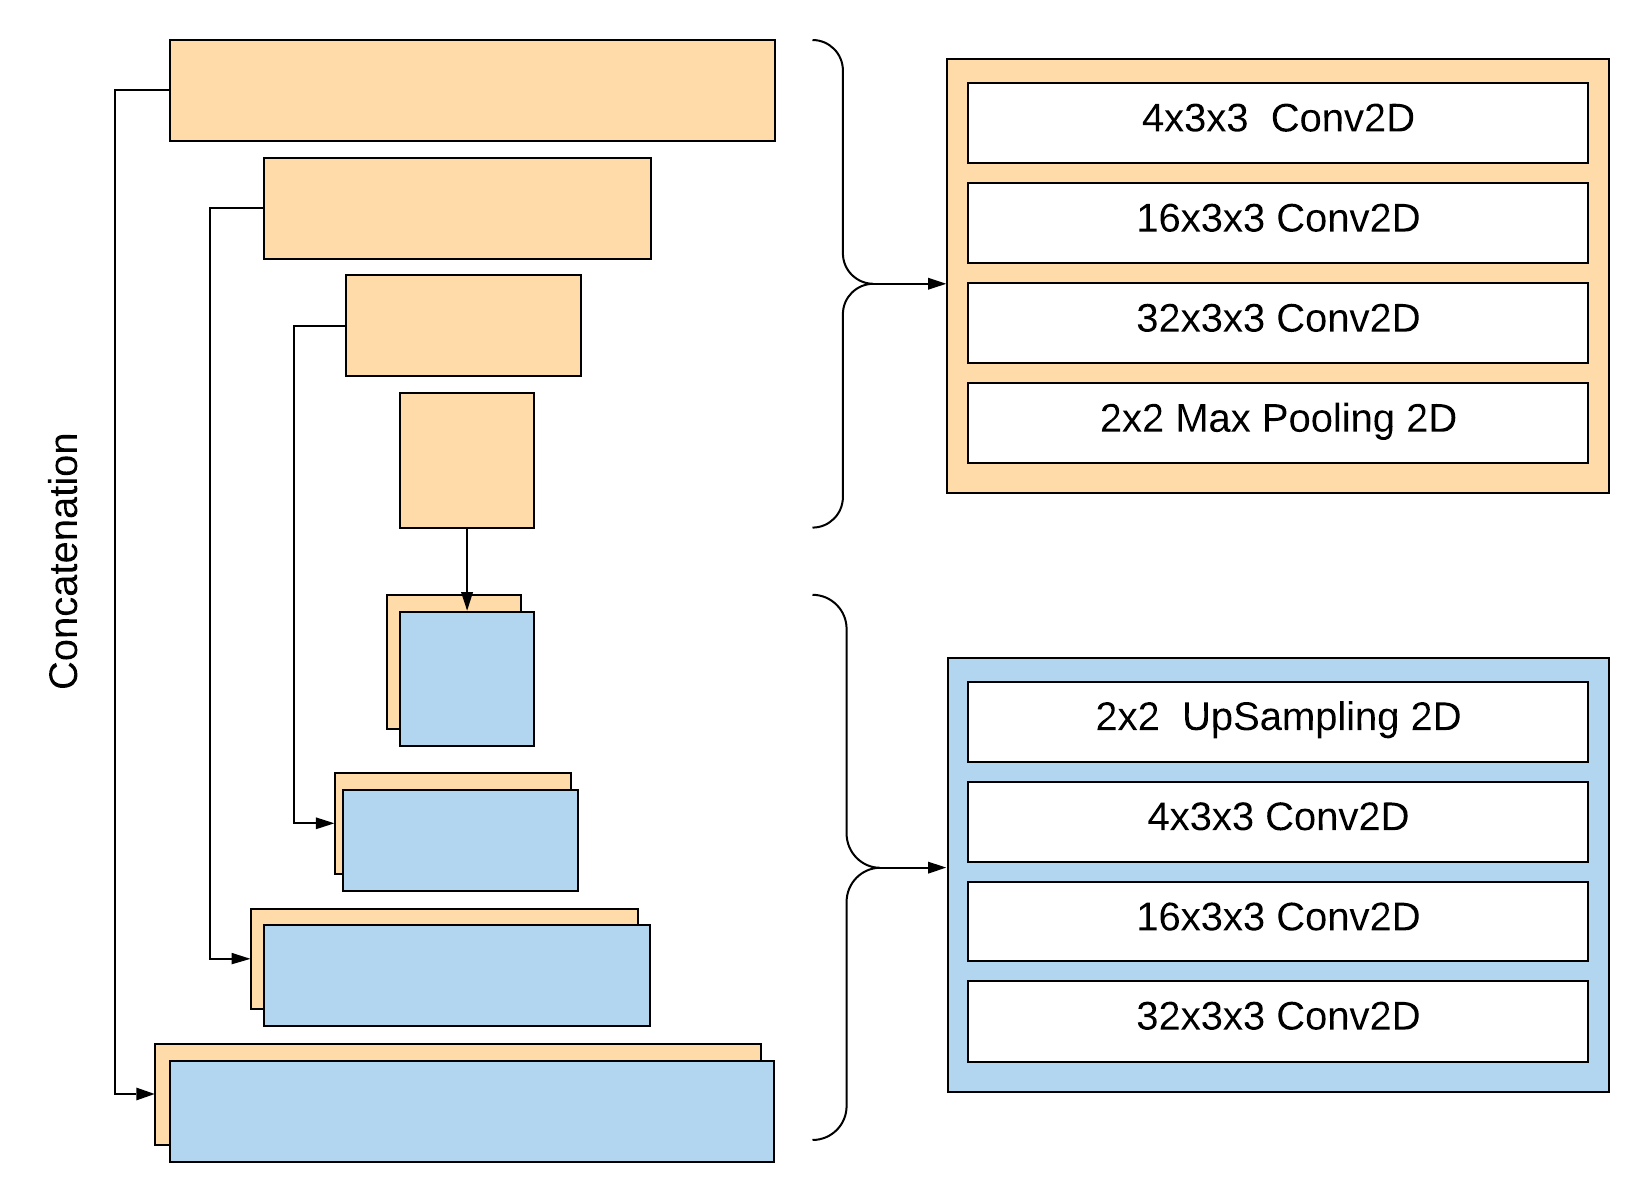
\includegraphics[width = 12cm, height = 10cm]{Figures/A1.png}
    \caption{U-Net architecture (\textbf{A1}). The bottom 4 blue blocks represents the decoder and the above 4 block represents encoder. }
    \label{fig:A1-U-NetArchetecture}
\end{figure}{}

U-Net (\textbf{A1}) architecture as shown in Fig \ref{fig:A1-U-NetArchetecture} is built upon simple idea of using upsampling layer or de-convolution layer  \footnote{not to be confused with the nomenclature, there are various names for de-convolution such as up-sampling layers or transposed convolution layer used by tensorflow and keras (\url{www.tensorflow.org/})} for up scaling the learnt feature and regeneration of depth maps. The motivation for building \textbf{A1} is to evaluate the influence of backbone architecture which has learnt the structural characteristic from a given image as seen before in Section \ref{Chapter3:RelatedWork_NNModel}. Another reason for us to use such approach lies in the simple architecture which is faster to train. The decoder block comprises of transposed 2D convolution layers which have the same dimension as the kernel size of encoder block. This means number of layers in encoder and decoder are the same that's why the name U-Net. 

\textbf{A1} consists of 4 blocks of encoder and decoder part. Each block of encoder consists of 4 layers, 3 layers of 2D Convolutions and 2D max pooling layer of size 2$\times$2 at the end of each block. We designed the 3 convolutions layer with the increasing order of number of filter 4, 16 and 32 with kernel size of 3$\times$3. In the similar way in each decoder block we have 4 layers, starting with an up-sampling layer with kernel size if 2$\times$2 which means the up scaling of the image is in the factor of 2. Nearest neighbor interpolation method used by the up-sampling layer \footnote{\url{www.tensorflow.org/api_docs/python/tf/keras/layers/UpSampling2D}} implemented by keras layer. Towards the end each decoder block has 3 convolution 2D stacked in the similar way as encoder blocks. Each decoder block is concatenated with relative encoder block which has same dimension as shown in fig. \ref{fig:A1-U-NetArchetecture} with arrow marks. The dimension of encoder and decoder block output tensors are kept in same with respect to the width and height if the image input dimension. This can be achieved by having same kernel size of max pooling at encoder part and up sampling layer at decoder, hence the symmetry in the encoder and decoder layers. The last output layer comprises of Convolution 2D layer of 1$\times$1 with sigmoid activation. Also last layer has no stride to keep the dimension same as the input. 
This model has input dimension of (batch size$\times$480$\times$640$\times$3) and output dimension of (480$\times$640$\times$1) for both target RGB image and ground truth depth images. Total trainable parameters of this model is 42,821.



\subsection{Approach 2 (A2) - DenseNet backbone}

\begin{figure}[h]
    \centering
    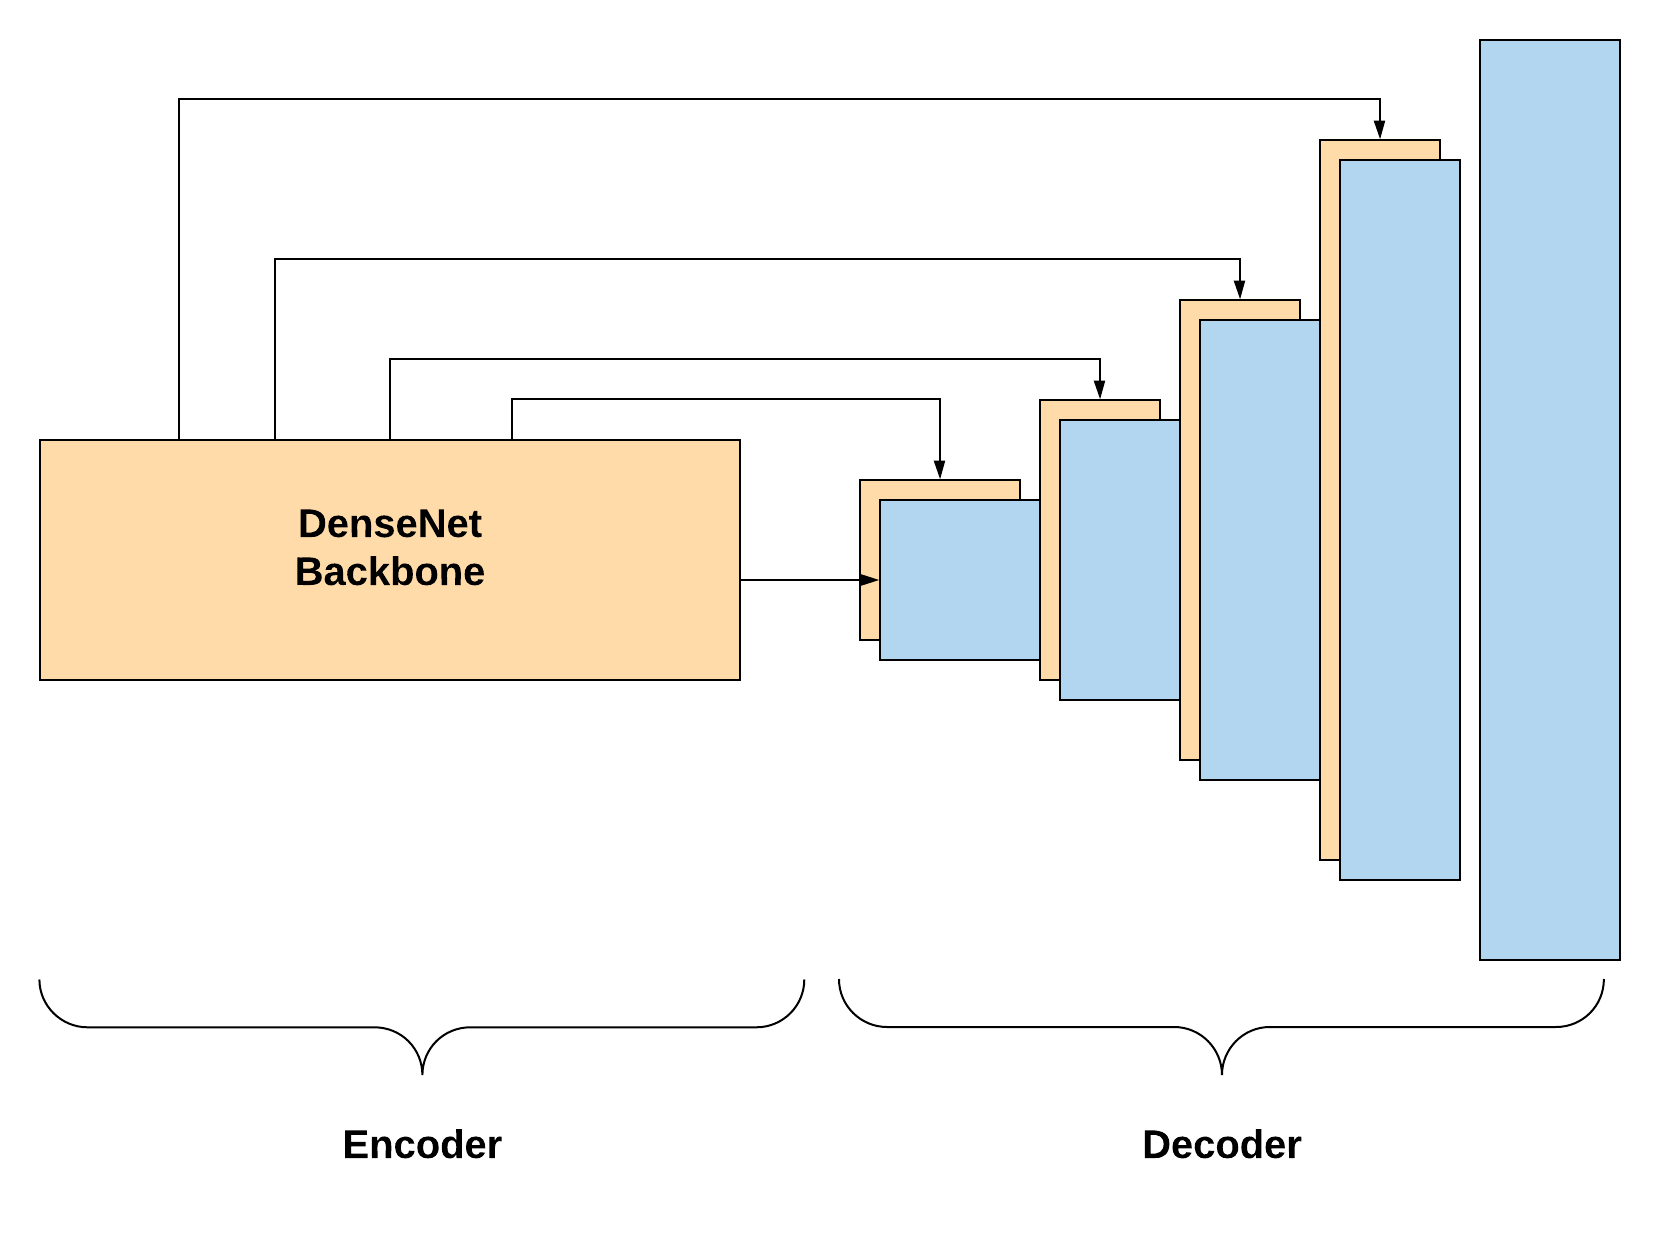
\includegraphics[width = 15cm,  height = 10cm]{Figures/A2.png}
    \caption{\textbf{A2} with DenseNet backbone}
    \label{fig:A2-DenseNet-arch}
\end{figure}{}




As shown in fig. \ref{fig:A2-DenseNet-arch} shows an overview of our second approach \textbf{A2} for depth estimation. We adapted the idea proposed by Alhashim et. al. \cite{Alhashim2018}. The basic idea of this approach \textbf{A2} was to use DenseNet as backbone or as an encoder from our literature study on this topic. The input RGB image is fed to the DenseNet-169 \cite{huang2017densely} network which is pretrained on ImageNet \cite{deng2009imagenet}.  Backbone DenseNet architecture is designed in a feed forward fashion within a dense block or in other words for feed forward design is that each layer is directly connected to every other layer. But since they adapt DenseNet style there is also skip connections between the layers. ImageNet is a large database of images which was build upon WorldNet which is organized in a hierarchical manner, which means the images are trained and clustered according to various classes which give a good hierarchical tree and sub-tree format for classification or clustering. Another great advantage of this net is its versatility of the classes ranging from mammals, vehicles, birds to furniture with 12 subtree which gives us 5247 category at the time of this paper by Deng et. al.\cite{deng2009imagenet}. ImageNet claims to have a order of 50 million images and an average of 5000 image per node \footnote{\url{http://www.image-net.org/}}. ImageNet is also good for object recognition, classification and also clustering problems. Due to such versatility, ImageNet can give us a good generalisation of the physical structure from a 2D image which is very important for our task. This also has proven to give state of the results by the model proposed by Alhashim et. al. \cite{Alhashim2018}. 


The design of this network is in such a way that the output from the DenseNet block is  fed to a successive series of up-sampling layers. The decoder has 5 Bilinear up-sampling blocks. \(4^{th}\) block is designed in a way that it give the output resolution half of its input, which is 230$\times$320$\times$1 for input size of RGB image 460$\times$640$\times$3. The \(5^{th}\) block has up-sampling factor of 2 which gives us full resolution same as input. In all our experiments we use only 4 blocks and in post processing we up sample by the factor 2 to get full resolution. This saves some computational time. The decoder part is trained on the 120,000 images of NYU v2 depth dataset. Also the decoder does not contain any Batch Normalization or other advanced sub multi task layers as seen in the recent state-of-the-art methods in section \ref{Chapter3:RelatedWork_NNModel}.

Each block of decoder comprises of 4 layers, starting with up-sampling by Bi linear with linear interpolation method. followed by concatenation operation and 2 convolutions 2D layers. The number of filters for these convolutions layer is decided by the number of filter obtained from the encoder layer which can be given by \(D_n =  {E_m} / {2^n}\) where \(D_n\) is number of filters at decoder block \(n\) and \(E_m\) is the number of filter present in the layer which is concatenated from encoder. The kernel size of these two convectional layers are of size (3$\times$3). The model proposed by  \cite{Alhashim2018} has target input dimension of 460$\times$640$\times$3 for RGB image and  dimension of 230$\times$320$\times$1 for ground truth label and we acquire the same principles for all our experiments. Also in the results section \ref{Chapter6:Results} we had some experiments by retraining the decoder part with different dataset and configurations to understand the influence of different. Total trainable parameters of this model is 42,657,689.



\section{Structure Depth Dataset Overview} 
\label{Chapter4:Dataset} 

Our aim in this work is to deliver a robust system for depth prediction as seen in the Figure \ref{fig:Proposed_Model} for a portable hand held mobile device. In our case it is an IPad integrated with Structure sensor. In order minimize the difference between the predicted depth maps and depth map generated from Structure sensor we need to train with the similar dataset. We have also validated this in our experiments which will be discussed below in Section \ref{Chapter6:Results}. As discussed in the Section \ref{Chapeter1:Topic_Description}, this will also help us to study the effect of different camera and sensor properties on different environment.\\

As we have seen earlier in Chapter \ref{Chapter3:RelatedWork}, there are multiple datasets available but almost none fit our context. As we are already exploiting the depth features from NYU V2 for general prediction, we would like to produce a dataset which is solely application based. Here our application is mobile device, particularly IOS, we generate the dataset using an IPad. This will not only make the intrinsic parameters to be learned by the network but also particularize for IOS based devices. As we use IPad as integration, all the RGB Images are received from the IPad's camera. The features we want the neural network to learn and predict should have the same camera intrinsic parameters in order to decrease the amount of pre processing of the dataset. Hence, We first calibrate IPad with Structure Sensor before collecting the Dataset. Another major advantage of using Structure Sensor with an IPad over Kinect is the resolution of RGB and Depth Images. While Kinect V2 has $512\times424$ Infrared camera resolution, Structure Sensor can go upto $640\times480$. \\

Our Dataset consist of two versions. The first version(SD\_v1) which was taken during the training of \textbf{A1} network which is detailed in Section \ref{Chapter5:Methodology}. In SD\_v1, we produced no hole depth images with wall of threshold 4 m. Since the temporal resolution of Structure Sensor is as high as 60 fps, there is not much difference in frames. So, in order to achieve a quality dataset, we saved a frame in every 10\textsuperscript{th} frame. Having a 60 fps video stream, we saved 6 fps. This removes redundant data and prevents us from over fitting the network. In the second version(SD\_v1) of our dataset, we captured every 2\textsuperscript{nd} frame per second giving us a temporal resolution of 30 fps. In SD\_v1, we removed the distance threshold and filled it with holes instead. We trained \textbf{A2} network with the new dataset. Including SD\_v1, we have a total of 18 scenes and consisting of \textbf{2675 images} captured using an Apple iPad Pro version 12.9 (2015) model and a Structure Sensor only. The dataset majorly includes images from office and classrooms environments. It consist of RGB Images of $640\times480$ as 3 channel $\times$ 8 bit int and Raw Depth Images of 640 $\times$ 480 as 1 channel. Both of the images are saved using lossless compression. Later, we also perform some processing to synchronize RGB and depth images and to fill the holes of depth image which will be discussed later in this chapter. We also provide the camera extrinsic parameters as a numpy matrix of $4\times4$ which is useful for reconstruction of a scenario.\\



\subsection{Technical Specification of Structure Sensor}
The Structure Sensor \footnote{\url{https://structure.io/}} is a 3D scanner introduced by Occipital in 2014. As the name suggests, it uses Structured-Light-System (SLS) 3D scanning\cite{Kalantari}. It can be easily attached to an IPad and with Structure SDK it enables us to generate good quality RGB image stream from IPad and its realtive depth stream from Structure Sensor at the simultaneously. As it only weighs 95 grams and can be used as an extension to mobile device, it makes the sensor very portable. With possibility of recording 60 frames per second at a resolution of $640\times480$\cite{Kalantari}. When compared to Kinect V2, it has more depth image resolution. The comparison can be seen in table \ref{table:KinectVsStructureSensor}. The minimum range it can capture is 40 cm while it can capture till 4 m with fine precision. After 4 m the precision is not satisfactory enough to use it for the dataset. Occipital claims it has low frame-to-frame noise and provides 100\% fill rate on most of the materials. On the other hand IPad Pro 12.9 provides us with an RGB video stream of $1920\times1080$ at 30 frames per second and $1080\times720$ at 60 frames per second. IPad Pro also provides us with Camera extrinsic parameters which are useful for the reconstruction of the scenario.\\

\begin{table}[h]
\begin{tabular}{@{}lll@{}}
\toprule
\textbf{Features}                    & \textbf{Kinect V2}           & \textbf{Structure Sensor}         \\ \midrule
Depth Sensor Type           & ToF & SLS                 \\
RGB Camera Resolution       & $1920\times1080$, 30 fps & $1920\times1080$, 60 fps     \\
IR Camera Resolution        & $512\times424$, 30 fps   & $640\times480$, 60 fps                 \\ 
Field of View of IR Camera  & $70^\circ\times60^\circ$           & $58^\circ\times45^\circ$                         \\
Recommended Operative Range & 0.4 m - 3.5 m       & 0.4 m - 3.5 m                                  \\
           &                     & 
\end{tabular}
\caption{Comparison of Kinect V2 and Structure Sensor}
\label{table:KinectVsStructureSensor}
\end{table}

\begin{figure}[h]
    \centering
    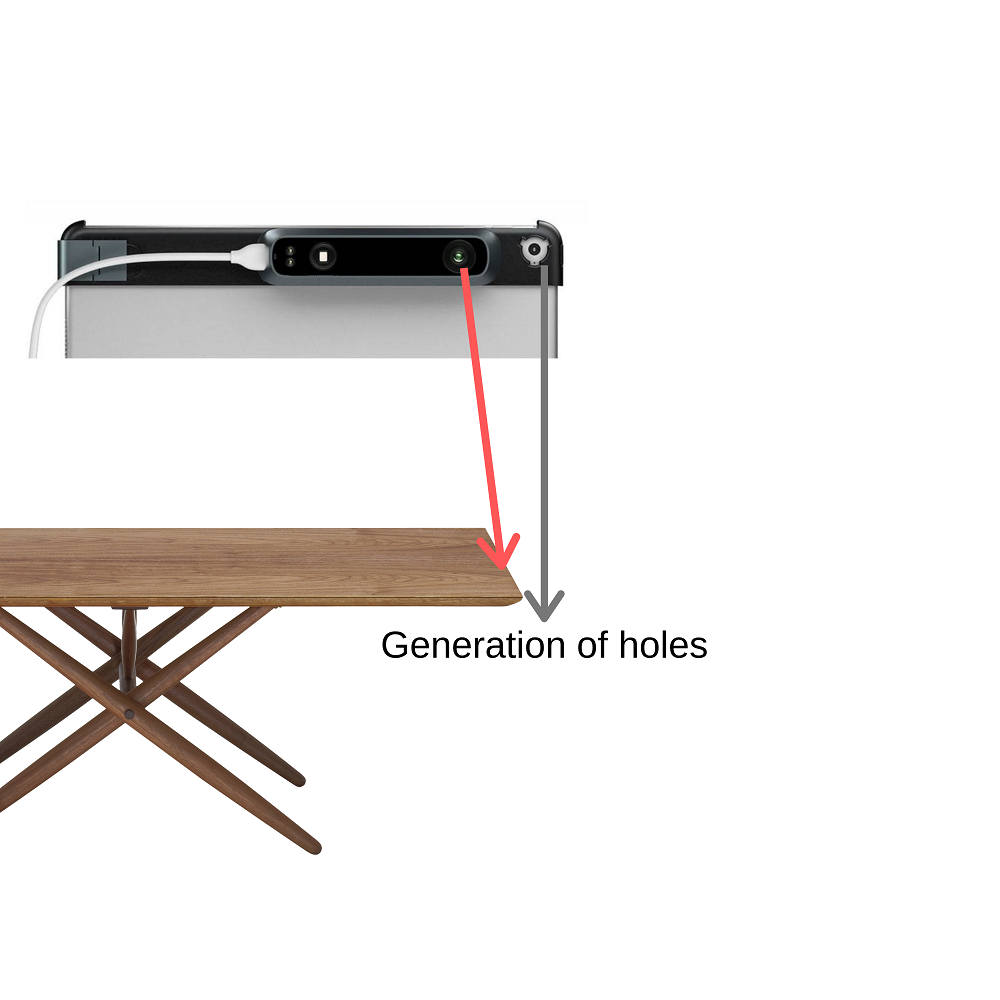
\includegraphics[scale=0.4]{Figures/holes.png}
    \caption{Generation of holes due to parallax}
    \label{fig:holes}
\end{figure}
While these sensors are great devices they have some limitations. The distance they can measure is limited and they suffer from reflection problems on transparent, shiny or very matte and absorbing objects. Another limitation is holes generated by parallax effect happening due to difference in position of the camera of IPad and Structure Sensor\cite{Kalantari}. In simpler terms, it works like human eyes. If we look at an object using only either of our eyes, we could notice disparities. When there is an object we try to focus on, our eyes which located at different position like the sensors in the Structure Sensor, they will see the object from different angles. If the object is close enough, then sometimes one eye can see what is behind and other can not. This can be seen in figure \ref{fig:holes}. As a result, it produces a shadow of holes which can be seen in figure \ref{fig:holes2}.



\begin{figure}[!]
\centering
    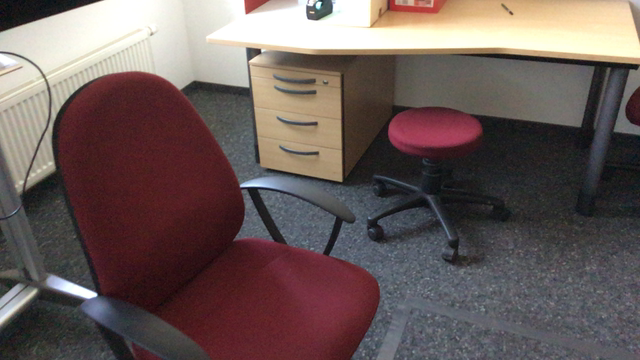
\includegraphics[scale=0.29]{Figures/RGB.png} 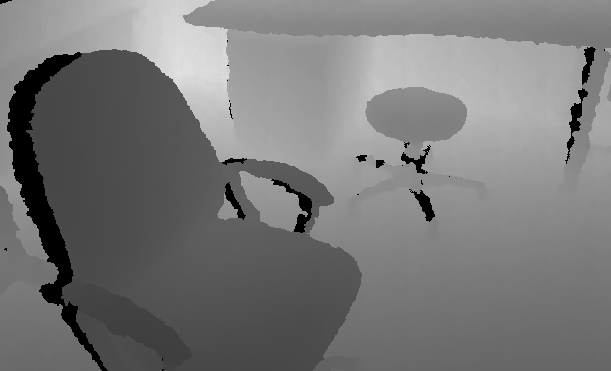
\includegraphics[scale=0.37]{Figures/Depth.png}
    \caption{Holes produced in depth image}
    \label{fig:holes2}
\end{figure}


\subsection{Dataset Collection}

A significant role in Machine Learning is played by Dataset and the collection of it makes most influence on the features that network learns. As the distance is limited in Structure Sensor and due to our scope of research we focus on indoor offices and classrooms environments. While capturing the dataset, one should keep in mind that the network should learn only the novel features not the artifacts. One good instance of this would be capturing the depth of a screen. Since, a screen has reflective black surface, it loses depth information resulting holes in depth image as seen in Figure \ref{fig:screens}. If we feed these images to the network, it might learn the features such as, screen is always at, let say x distance, where x is pixel value we assign to such holes. These holes are the undesired features and called artifacts. Such artifacts could be produced due to various reasons. It could be the reflective/absorbing nature of the surface of an object or the distance and position of the object\cite{geomar41830}. As a reflective/glossy surface leads us to wrong or no generation of depth pixel, we try to avoid them while capturing. Figure \ref{fig:screens} is one good example of such holes. As we notice in the RGB image there are two screens, one is predicted in some regions while other one is totally lost. In indoor environments, such objects are inevitable. Thus, in such problems we use techniques like inpainting \cite{inpainting}. Image inpainting could also be used to resolve artifacts due to parallax effect discussed in section previous section.\\
\begin{figure}[h]
    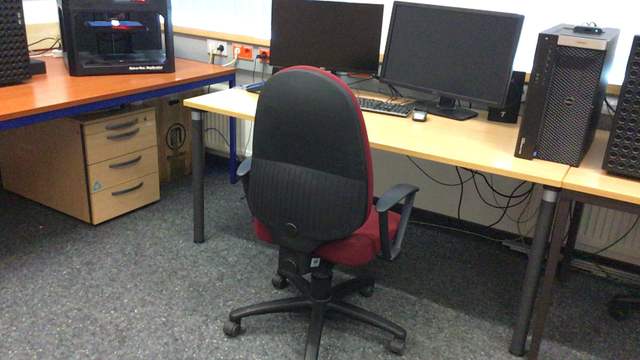
\includegraphics[scale=0.29]{Figures/7.png} 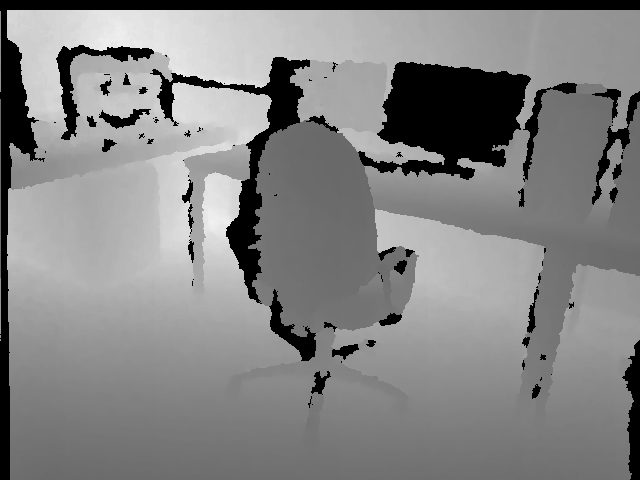
\includegraphics[scale=0.24]{Figures/Raw7.png}
    \caption{Holes produced in depth image due to reflectivity of the screen}
    \label{fig:screens}
\end{figure}
 

Since, the accuracy decreases with the increase in depth \cite{deptherror} and because the recommended range is no more than 4 metres(m) for Structure Sensor \cite{Kalantari}, we remove all the pixels which are far away than 4 m. These pixels can be resolved using further predictions and post processing. This also protects our network from learning the artifact of distant objects as a wall as discussed in \ref{Chapeter1:Topic_Description}.\\

\subsection{Data Processing}

The very first step of processing the dataset would be registering the depth pixels. After we have calibrated the camera, we convert the pixels received from Structure Sensor to millimetres(mm) for ease of understanding as the pixel value have a non linear relationship. After we have the distances in metres, we want to eliminate all the possible artifacts as these images still contain holes and precision less pixels. Usually, far away pixels have less precision and results in holes as well\cite{deptherror}. It is a good idea to conserve those pixels as holes in order to reconstruct the environment by later predicting the future frames. Firstly, after we have the depth images in metres, we save all the holes by its pixel position or index for all the pixels more than 4000 mm so that we can use that information later. By doing so, we can eliminate the distance threshold artifact discussed earlier.

\begin{figure}[!]
    \centering
    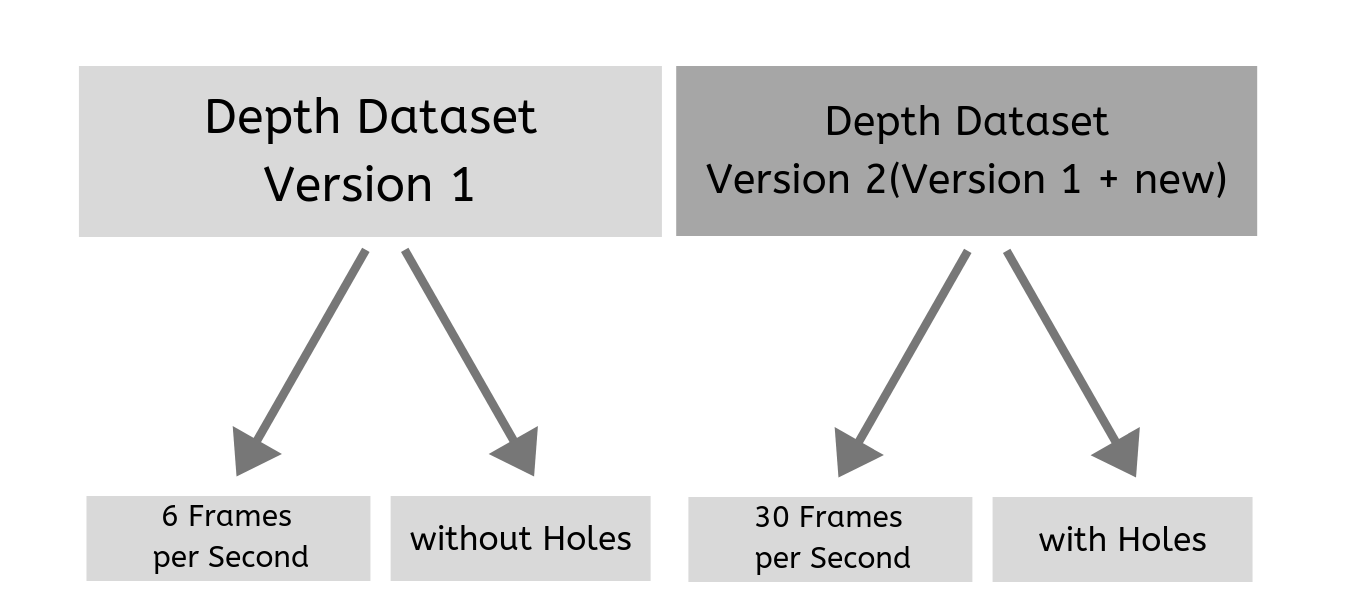
\includegraphics[scale=0.35]{Figures/versions.png}
    \caption{Versions of our proposed dataset}
    \label{fig:datasetversion}
\end{figure}

\begin{figure}[h]
    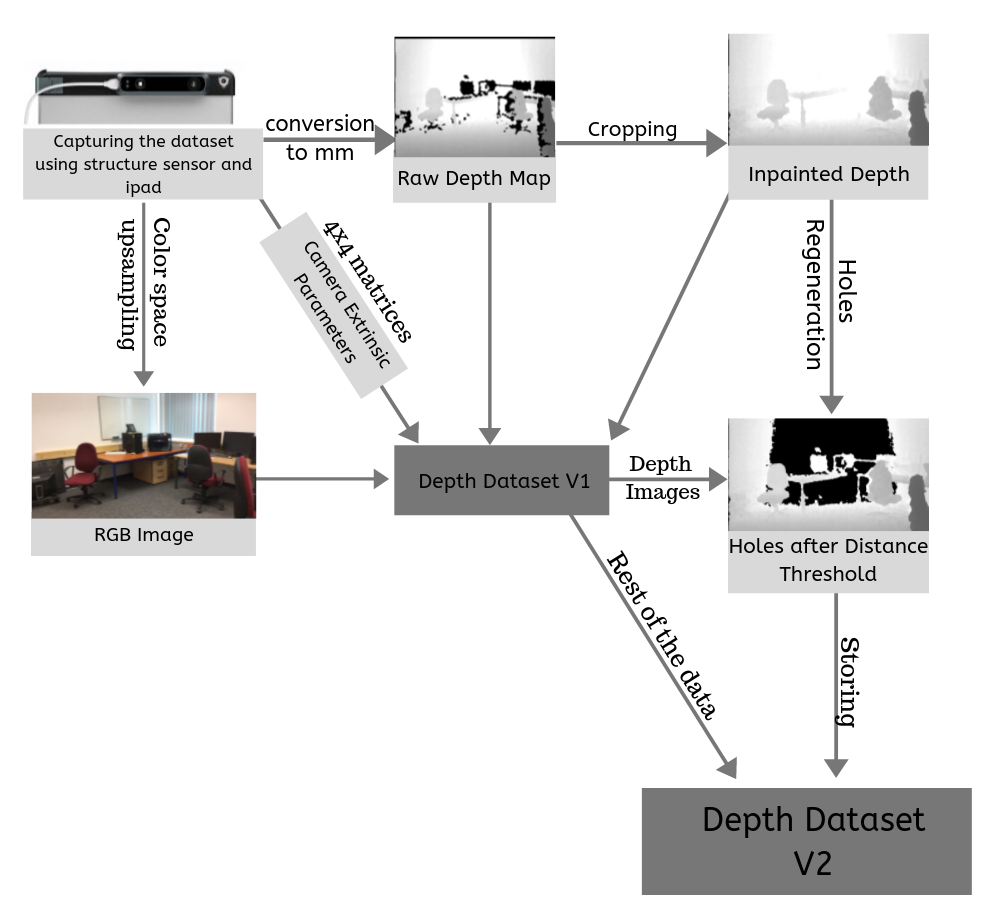
\includegraphics[scale=0.50]{Figures/process.png}
    \caption{Different stages of processing the depth frames}
    \label{fig:processing}
\end{figure}

As discussed earlier, the Depth images contains holes from shiny/glossy objects\cite{shiny}. In office environments, these holes are mostly generated by Computer Displays. Since we do not want our network to learn that all the screens are close(0 pixel), we interpolate these holes. We do this by inpainting \cite{inpainting} the whole image. This fixes the issues of shadows produced due to the parallax as well. Noting that it inpaints the pixels more than 4 m too. SD\_v1 of our dataset consisted of depth images which were totally inpainted and there were no holes as can be seen in \ref{fig:datasetversion}. Basically which means, if some of the pixels which are far away than 4 m are missing, they are interpolated using nearest neighbours. As we know, these predictions are not very accurate from past discussion, it is also possible that the inpainted depth is not correct. So In SD\_v1, successor of SD\_v1, we use the index of pixels of depth more than 4 m we saved now later in the process. This will reproduce all the holes which were more than 4 m as missing information is better than wrong predictions. These holes can later be predicted using the future frames. Our depth image is now ready to be fed to the network but as one would have noticed before, The size of the Color Image and Depth Image does not match since they have different aspect ratios due to different camera sources. So, In the end we crop the depth image centre focused in order to make them compatible with the network. We can understand this through Figure \ref{fig:processing}, where we show how the captured data and is processed and stored. \\



\newpage
\section{System Setup}
\label{Chapter5:Experimental_Setup}
\subsection{Training and Experimental Configurations}

 Our entire experimental experimental configuration are described in the fig \ref{fig:Experimental_Setup}. All the configuration where made based on two model \textbf{A1} and \textbf{A2} and two data pre-processing \textbf{Holes} and \textbf{No\_Holes}. Added to this we also did a \textbf{transfer learning} over \textbf{A2} by retraining the model with Structure Sensor dataset. This gives two models and five different configuration to analyze foe our study. 


First, Our proposed model \textbf{A1} is a simple U-Net style architecture - also can be categorized as encoder-decoder style of architecture. There are two specific reason for designing simple architecture. (a) To understand if a simple network can learn the feature from a given depth image. one of the advantage of a simple small network is we have faster computation for the implementation (b) If a new architecture can learn without any prior knowledge of such structures, if yes how well can it perform. This motivated us to evaluate our model performance against an existing model.As previously discussed in the Chapter \ref{Chapter3:RelatedWork}  where chose approach \textbf{A2} proposed by Alhashim et. al. \cite{Alhashim2018}. Also developing \textbf{A1} involved various network configuration parameter optimization only the final best working model has been documented in the Section \ref{Chapter5:A1}. \\

Secondly, we wanted to investigate if dataset from different sensor with different cameras intrinsic and extrinsic properties can influence our results.  This result was necessary because our study is to answer if we can replace structure sensor by neural network, thus we have structure dataset to get as close results as structure sensor. This experiment also gives us a good validation base if there is a need for task and hardware based dataset for neural network models to perform on cross platform environment - in our case  the cross platform environment would be between neural network trained kinect dataset and mimicking Structure Sensor. For this our idea was to train our model with two dataset NYU\_v2 depth dataset and structure depth dataset. We train only the decoder block of \textbf{A2}. Alhashim et. al \cite{Alhashim2018} model was trained on 120,000 images from NYU\_v2 dataset and these weights for decoder block was publicly available. Therefore we call this experiment setup as \textbf{Transfer Leaning} approach. Hence we had two experiments, one by evaluation the model trained on  datasets from kinect sensor and another trained on both kinect and structure. By using the pre-trained weights, it saves computational time and memory while different training and experimental configuration. \\

Thirdly, we wanted to investigate if a model can learn the holes generated from the SLS sensor. In our literature study in Section \ref{Chapter3:RelatedWork} most of the work where based on approach where the depth data was processed  in a way where the holes where interpolated. The most common and widely used method was to either in-paint (or fill) the holes using neighboring pixel \cite{silberman11indoor} method. We approached this problem by saving the holes and map all the invalid holes to zero value instead of finding neighboring pixel which was used in NYU dataset. We trained \textbf{A2} model in two different fashion. One by mapping the holes to a zero value we call it as \textbf{A2\_Holes} and another we find the neighboring pixels and we call this approach as \textbf{A2\_NoHoles}.

\begin{figure}[h]
    \centering
    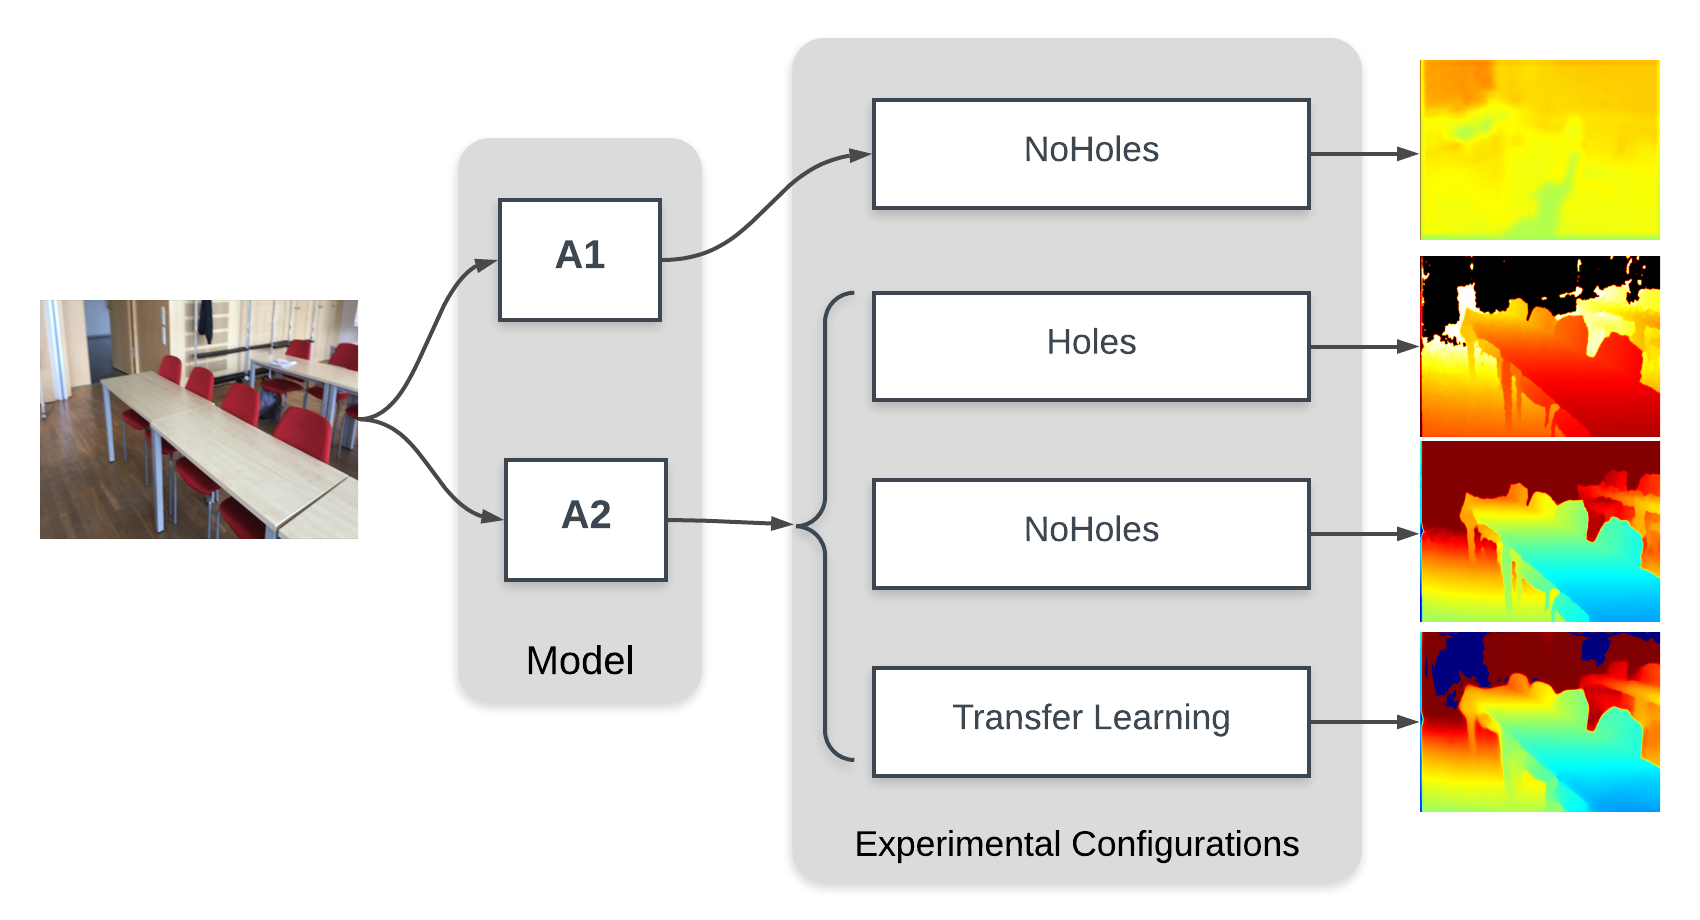
\includegraphics[width = 14cm]{Figures/config_setup.png}
    \caption{Different experimental configuration were setup based on \textbf{A1} and \textbf{A2} approaches}
    \label{fig:Experimental_Setup}
\end{figure}{}

Finally, we wanted to investigate the best working configuration to evaluate against a baseline model on the test set of Structure Sensor. 

Therefore in summary, we have two model \textbf{A1} and \textbf{A2} for validating the proposed model and effects of structural Characteristic. Further more \textbf{A2} model where retrained with two different modified input features for investigating on regeneration of holes. This gives us two more configuration of \textbf{A2} model namely \textbf{A2\_Holes} and \textbf{A2\_NoHoles}. These four configuration where made to fit the three different experimental conditions. First experiment is based on changing parameters with respect to encoder to see if the influence of backbone. second experiment is based on changing parameters at decoder where we analyze the influence of different camera properties by training with different dataset. Third is by evaluating against two dataset configurations .

\subsection{Loss Function}
\label{Chapter5:LossFunction}
A standard loss function for depth estimation problems is computed by finding the difference in predicted values \(\hat{y}\) and truth \(y\). In our work we use loss function proposed by \cite{Alhashim2018}. One of the significe of this loss function is, it not only computes difference in t \(\hat{y}\) and truth \(y\) acting as minimizing error function but also it focus on higher frequency penalizing. The reason for having weight for higher frequency of an image is to compute the performance of the network corresponding to the object boundaries. The resultant loss function \(L\) is computed as a weighted sum of three loss functions which are pair wise loss \(L_{depth}\), image gradient loss \(L_{grad}\) and structure similarity loss  \(L_{SSIM}\) which is given by:


\begin{equation} \label{eq:loss}
       L(y, \hat{y}) = \lambda_{1} L_{depth}(y, \hat{y}) + \lambda_{2} L_{grad}(y, \hat{y}) + \lambda_{3} L_{SSIM}(y, \hat{y})
\end{equation}




%%%%%%%%%%%%%%%%%%%%%%%%%%%%%%%%%%%%%%%%%%


%\begin{itemize}
 %   \item First the pare wise depth is given by:
%\end{itemize}{}
\begin{equation} \label{eq:loss_depth}
      L_{depth}(y, \hat{y})= \frac{1}{n} \sum_{p}^{n} \left|y_{p} - \hat{y}_{p} \right|
\end{equation}

First the pare wise depth is given by euation \ref{eq:loss_depth}. This gives us a pixel level understanding of error between ground truth and predicted image.  
%%%%%%%%%%%%%%%%%%%%%%%%%%%%%%%%%%%%%%%%%%

%\begin{itemize}
%    \item Structure similarity loss
%\end{itemize}{}
\begin{equation} \label{eq:loss_grad}
       L_{grad}(y, \hat{y}) =  \frac{1}{n} \sum_{p}^{n} \left| g_{x} (y_{p} - \hat{y}_{p}) \right| + \left| g_{y} (y_{p} - \hat{y}_{p}) \right|
\end{equation}


Secound, the \(L_{grad}\), which computes the gradient changes with respect to its neighboring pixels. Here the image gradient \(g\) is computed in two directions \(g_{x}\) and \(g_{y}\) which compute the differences in \(x\) and \(y\) component of the depth images. \\


\begin{equation} \label{eq:loss_SSIM}
       L_{SSIM}(y, \hat{y}) = \frac{1- SSIM(y, \hat{y})}{2}
\end{equation}

Third, the Structrural Similarity Index (SSIM) proposed by Wang et. al. \cite{wang2004image} gives us a good understating of groups of pixel based of comparative measure of three components individually which are luminance, contrast and structure similarities between ground truth and predicted. The final \(L_{SSIM}\) is a reciprocal version of SSIM as in \cite{Alhashim2018,  ummenhofer2017demon, huang2018deepmvs}.
%%%%%%%%%%%%%%%%%%%%%%%%%%%%%%%%%%%%%%%%%%


%\begin{itemize}
%    \item Image gradient loss:
%\end{itemize}{}


We used tensorflow implementation of \(L_{grad}\) \footnote{\url{https://www.tensorflow.org/api_docs/python/tf/image/image_gradients}} and \(L_{SSIM}\) \footnote{\url{https://www.tensorflow.org/api_docs/python/tf/image/ssim}}  in our study \cite{tensorflow2015-whitepaper}. Though out the experiments the weightage factor for our loss function in equation \ref{eq:loss} where set to  \(\lambda_{1} = 0.1, \lambda_{2} = 1, \lambda_{3} = 1\) suggested by \cite{Alhashim2018}. Hence we try to supervise our network based on structural similarities more than pixel level similarities. 


\newpage

%From the above equation \ref{eq:loss} The 

\subsection{Evaluation Metrics}
\label{Chapter5:Evaluation_mat}
For our evaluation we use standard metrics used in prior work \cite{Alhashim2018, eigen2014depth}. The error metrics are defined as follows:
%%%%%%%%%%%%%%%%%%%%%%%%%%%%%%%%%%%%%
\begin{itemize}
    
    \item Root Mean Squared Error (RMSE):
    
\end{itemize}{}

\begin{equation} \label{RMSE}
        \sqrt{\frac{1}{n} \sum_{p}^{n}{(y_{p} - \hat{y}_{p}})^2}
\end{equation}
%%%%%%%%%%%%%%%%%%%%

\begin{itemize}

    \item Average (${log_{10}}$) error: 
    
\end{itemize}{}

\begin{equation} \label{avg_log}
    \frac{1}{n} \sum_{p}^{n} \left|log_{10}(y_{p}) - log_{10}(\hat{y}_{p}) \right|
\end{equation}

%%%%%%%%%%%%%%%%%%%%%%%%%%%%%%%%%%%%%%

\begin{itemize}
    \item Threshold Accuracy (\(\delta_{i}\)): 
\end{itemize}{}

\begin{equation} \label{ThresholdAcc}
    {\delta = max (\frac{{y_{p}}}{\hat{y_{p}}}, \frac{\hat{y_{p}}}{{y_{p}}})}
\end{equation}

The threshold accuracy is computed based on 3 different threshold values which are given by \(\delta < a_{i}\)  \(a_{1}= 1.25^1, a_{2} = 1.25^2, a_{i} = 1.25^3\)  
%%%%%%%%%%%%%%%%%%%%%%%%%%%%%%%%






\subsection{Implementation Details}
\label{Chapter5:HardwarSoftwareDetails}
%ECCRTX-OPS 84T 
Here we mention all the necessary tools and modules used in this study. 

 \subsubsection{Training Configurations} 
 \label{Chapter4:TrainConfigurations_i}

 Though out all our  experiments we trained all our model for 1000 epoc with an early stopping of 10. We used Adam \cite{kingma2014adam} optimizer with the learning rate of \(10^{-4}\). For loss function and evaluation metrics we use methods as described in Section \ref{Chapter5:LossFunction} and Section \ref{Chapter5:Evaluation_mat} respectively.
 
 \subsubsection{Dataset} 
  \label{Chapter4:DatasetForsplits-i}

 We used two dataset they are NYU\_v2 and and two versions of Structure depth dataset (SD\_v1 and SD\_v2) datasets. NYU\_v2 is publicly available and SD\_v1 and SD\_v2 were created for this task. For all the experiments we used 80-10-10 (\%) split for training, validation and test set. We had one test sets for each of the dataset. For NYU\_v2 we used standard test set available online comprising of 1449 RGBD images. Similarly for SD dataset we used a total of 2675 RGBD images.
 
\subsubsection{Hardware} 
\label{Chapter4:Hardware_i}
For all our experiments we used \textit{Nvidia Quadro RTX 8000} \footnote{\url{https://www.nvidia.com/content/dam/en-zz/Solutions/design-visualization/technologies/turing-architecture/NVIDIA-Turing-Architecture-Whitepaper.pdf}} graphic card with Graphics processor GDDR6  having memory of 48 Gigabyte on Linux operating system with Ubuntu distribution 18.04. For capturing dataset, we used Apple iPad Pro version 12.9 (2015) integrated with Structure Sensor by Occipital with the help of Structure Software Development Kit.


\subsubsection{Software} 
\label{Chapter4:Software_i}
For the implementation of Neural Network model and related tasks, we used Keras 2.2.4 framework with Tensorflow 1.13.1 \cite{tensorflow2015-whitepaper} backend for python environment \footnote{\url{www.python.org}}. CUDA 10.1 (a software layer which gives direct access for multiple processing on GPUs having two main key attribute of hierarchical multiprocessing thread groups and shared memory \cite{nickolls2008scalable}) the GPU  the above mentioned  \textit{Nvidia Quadro RTX 8000} graphic card. Additionally, we used openCV library \cite{opencv_library} for varous image processing tasks. For dataset collection, we used Xcode 10.2 \footnote{\url{https://developer.apple.com/documentation/xcode_release_notes/xcode_10_2_release_notes}} to send the data over the network in bit stream. The data was retrieved and processed using python environment.


\subsubsection{System Computational Efficiency}

Here we would like to report our neural network model computational efficiency in the table \ref{table:ModelComputationaleff}. These measure are with respect to time in seconds for loading of a model  and prediction on test set comprising of 271 image from SD\_v2 dataset.

% Please add the following required packages to your document preamble:
% \usepackage{multirow}
% Please add the following required packages to your document preamble:
% \usepackage{multirow}
\begin{table}[!]
\centering
\begin{tabular}{|c|c|c|c|c|c|c|c|}
\hline
\multicolumn{2}{|c|}{\textbf{Model}}      & \textbf{1} & \textbf{2} & \textbf{3} & \textbf{4} & \textbf{5} & \textbf{Mean} \\ \hline
\textbf{A1} & Load Model & 2.6        & 2.6        & 2.7        & 2.7        & 2.6        & \textbf{2.6}  \\ \cline{2-8} 
                             & Prediction & 25.8       & 25.4       & 26.2       & 26.5       & 26.2       & \textbf{26.0} \\ \hline
\textbf{A2} & Load Model & 47.3       & 48.2       & 46.2       & 45.5       & 47.1       & \textbf{46.8} \\ \cline{2-8} 
                             & Prediction & 44.9       & 45.7       & 44.3       & 42.6       & 41.8       & \textbf{43.8} \\ \hline
\end{tabular}
\caption{\textbf{System Computational Efficiency}: All the above readings are in seconds. We run the model five times to take the mean time.}
\label{table:ModelComputationaleff}
\end{table}

\newpage



\section{Schedule and Milestones}
\begin{figure}[h]
\centering
    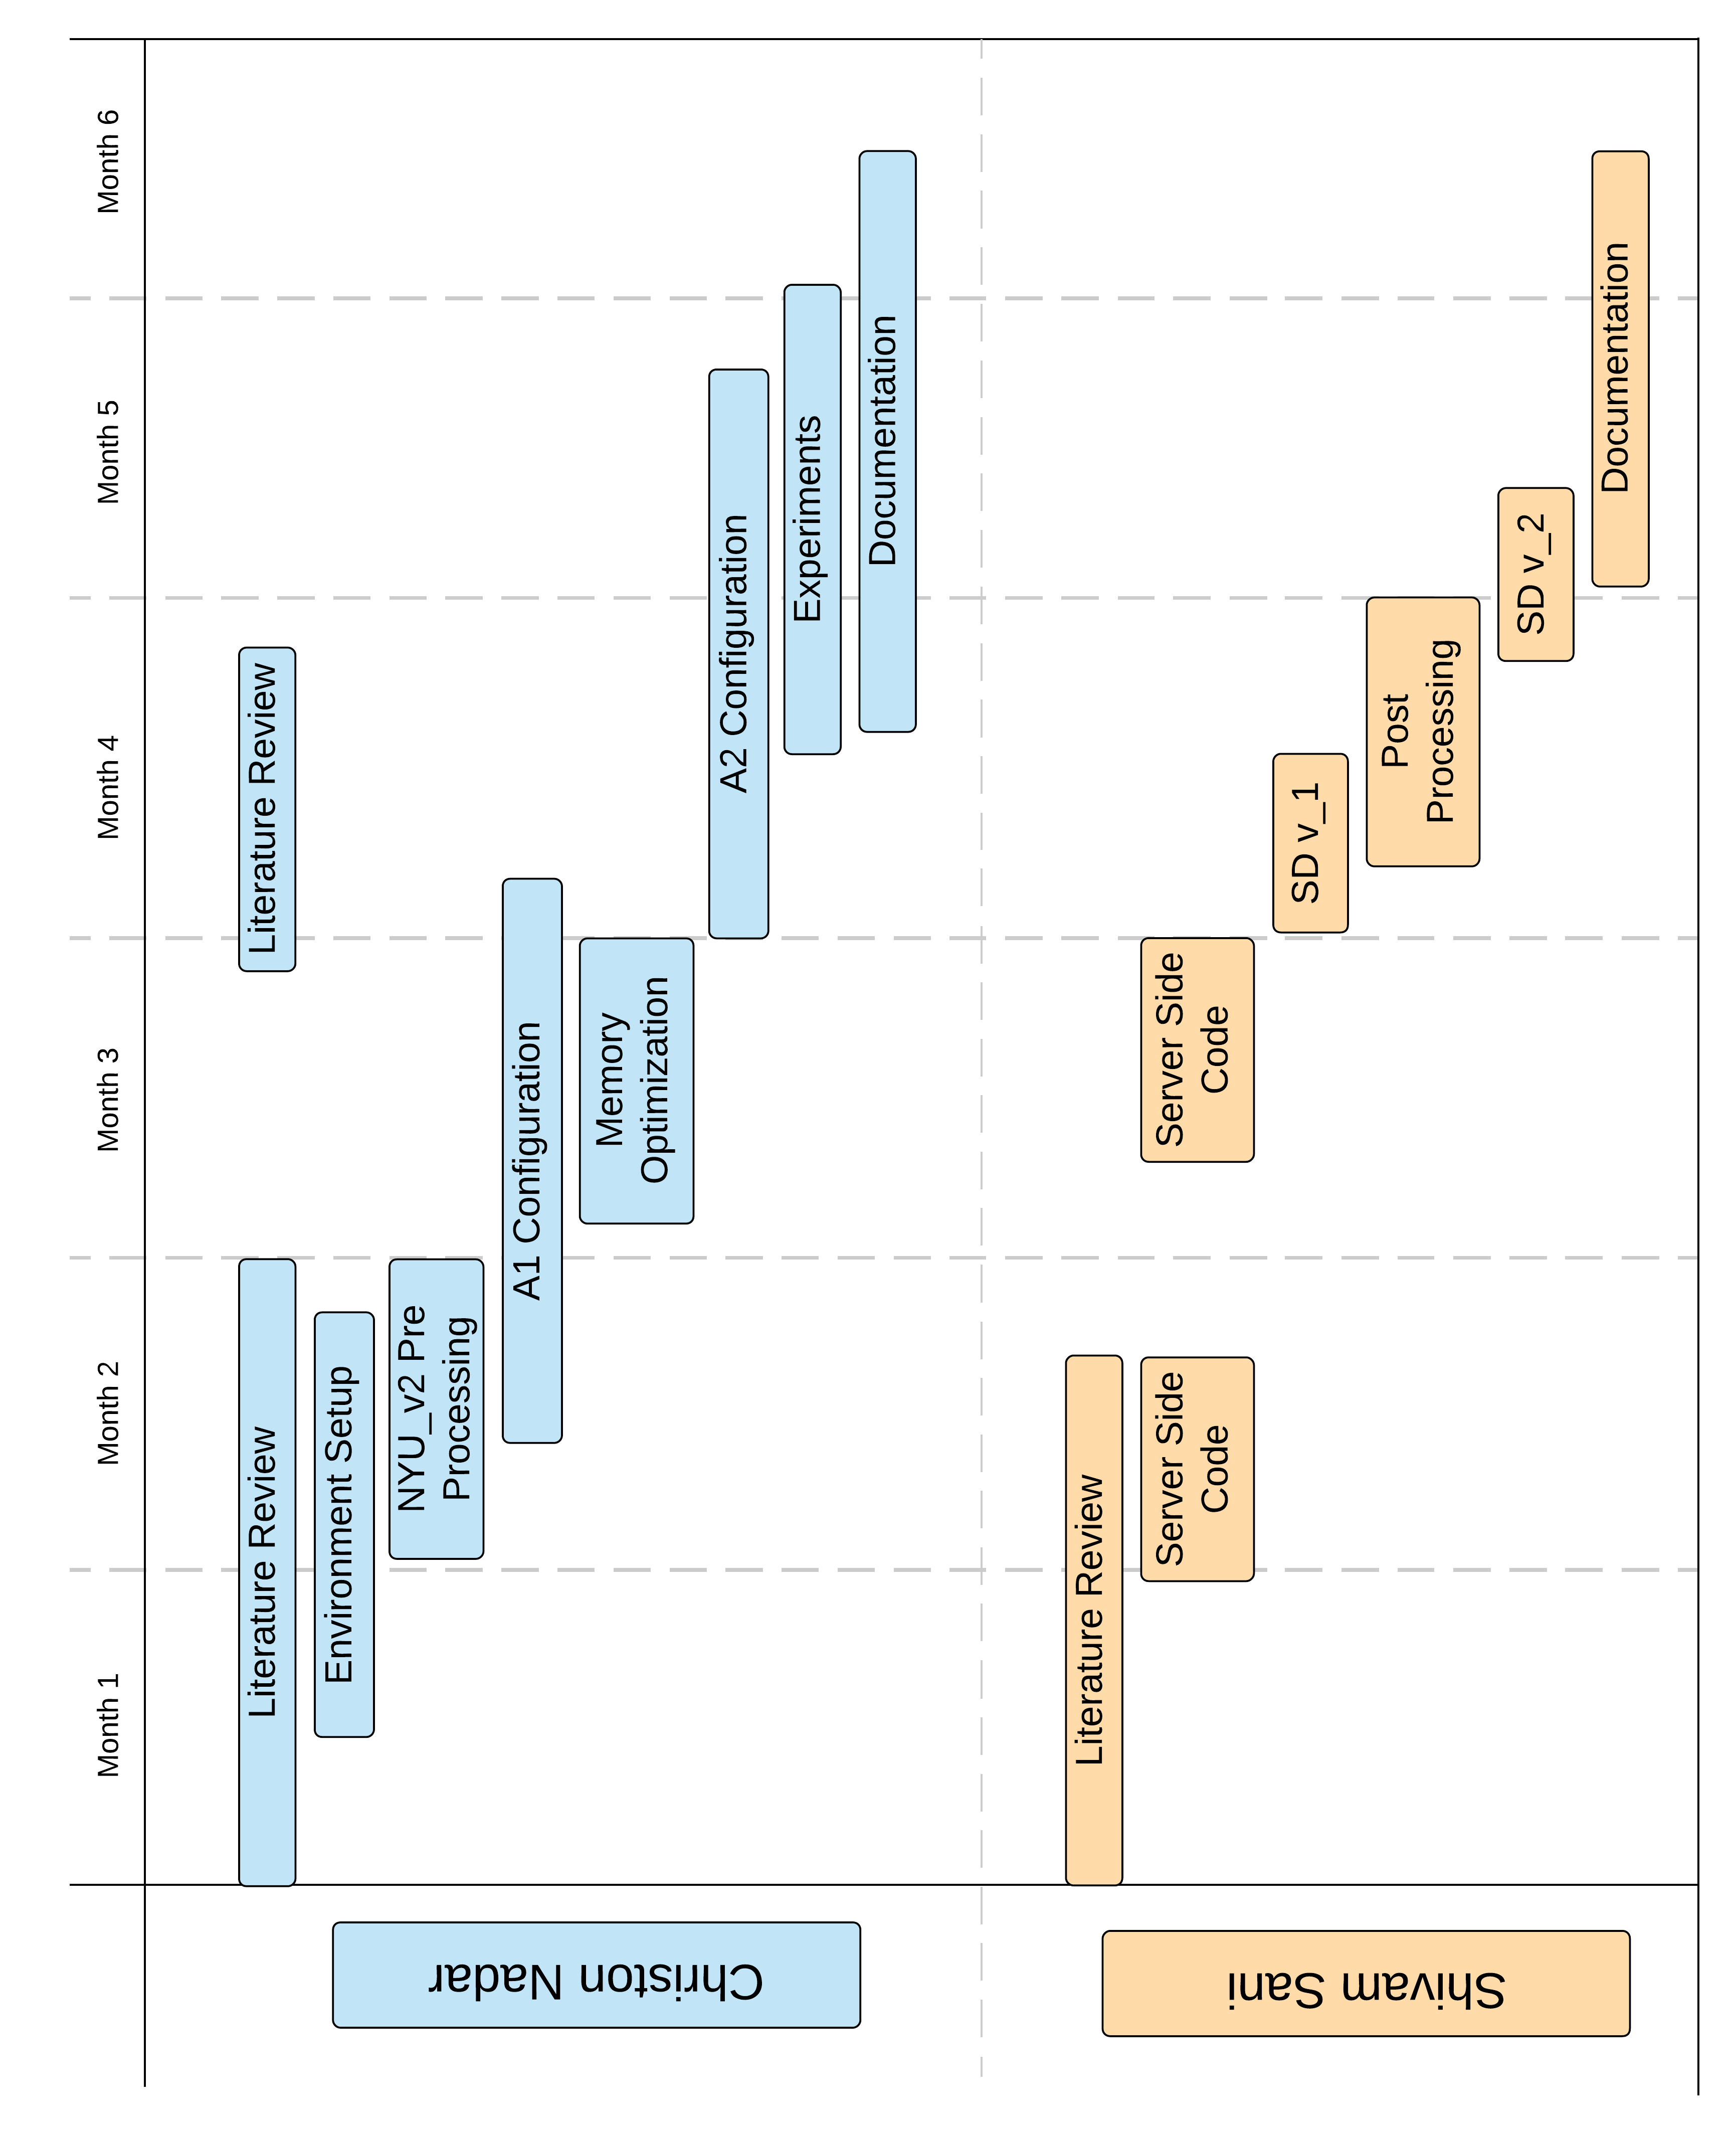
\includegraphics[width=14cm, height=18cm]{Figures/ganntL2.png}
 \caption{Gannt Diagram}
    \label{fig:Gannt_Dia}
\end{figure}
\newpage

